\chapter{实验评估}

本章将介绍针对\tool 所开展的实验评估,讨论并分析实验的结果。首先,本文从五个方面提出五个研究问题,包括准确性、削弱性、敏感度、通用性和实用性。然后,针对这五个问题再逐一评估,讨论并分析结果的原因及意义。最后,基于实验评估的结果,讨论\tool 的价值及局限性。

\section{实验问题设计}
本文从准确性、削弱性、敏感度、通用性及实用性五个方面设计了以下五个研究问题,以尽可能全面地评估\tool 。

\begin{itemize}[leftmargin=*]
\item \textbf{RQ6 准确性评估:}与已有的基于启发式规则的方法相比,\tool 识别漏洞补丁的准确性如何?与两个商业漏洞数据库相比,\tool 识别的漏洞补丁准确性又如何?这个研究问题旨在对比评估\tool 的准确性(见章节\ref{sec:accuracy-evaluation})。
\item \textbf{RQ7 削弱性分析:}\tool 中各个步骤及环节的设计有着怎样的效果?或有着怎样的必要性?如果去除\tool 中的某些环节,或削弱\tool ,对于最终结果会有怎样的影响?这个问题旨在评估\tool 中各个步骤及环节设计的实际效果及必要性(见章节.\ref{sec:ablation})。
\item \textbf{RQ8 敏感度分析:}\tool 对设计参数的敏感性如何?这个问题旨在评估\tool 的健壮性及鲁棒性,探究\tool 中的参数是否对结果的准确性有过大影响(见章节\ref{sec:sensitivity})。 
\item \textbf{RQ9 通用性分析:}\tool 在更大范围的开源软件漏洞上表现如何? 这个问题旨在评估\tool 的通用性(见章节\ref{sec:sensitivity})。
\item \textbf{RQ10 实用性分析:}\tool 在实际使用中表现如何?这个问题旨在评估\tool 在实际工作中实用性(见章节\ref{sec:generality})。
\end{itemize}

为解答以上研究问题,本章的实验评估将继续采用经验研究(见章节\ref{sec:accuracy})中的评估指标,即Coverage(覆盖率)、Precision(精确率)、Recall(召回率)和 F1-Score(F1值)。本章的实验评估还将继续使用在经验研究(见章节\ref{sec:study})中构建的深度数据集,以探究\textbf{RQ6 准确性评估}、\textbf{RQ7 削弱性分析}和\textbf{RQ8 敏感度分析}。

对于\textbf{RQ9 通用性分析},本文将另外构造两个更大范围的数据集来进行评估。此外,本文还进行了用户研究,通过分析用户在有和没有\tool 辅助下查找补丁的用时和准确性,并基于用户反馈,来探究\textbf{RQ10 实用性分析}。


\section{RQ6:准确性评估}\label{sec:accuracy-evaluation}

为了评估\tool 的准确性,本节将\tool 分别与三种基于启发式规则的方法和两个商业漏洞数据库($DB_A$和$DB_B$)进行比较,并进一步分析了\tool 中误报和漏报的原因。

\subsection{与基于启发式规则的方法对比}
本节首先选择了两种被广泛使用的基于启发式规则的方法(\textbf{检索NVD}\cite{duan2019automating,li2016vulpecker,li2018vuldeepecker} 和\textbf{检索GitHub}\cite{you2017semfuzz,Wang2020empirical}),此外,将这前两种方法结合为第三种基于启发式规则的方法(\textbf{检索NVD以及GitHub})。

\textbf{检索NVD:}检索NVD平台上该漏洞“Reference”字段中引用的参考链接以获取补丁提交。如图\ref{fig:CVE-2019-18841}所示为NVD平台上CVE-2019-18841的参考链接\footnote{https://nvd.nist.gov/vuln/detail/CVE-2019-18841},可以从中提取出补丁提交“https://github.com/ankane/chartkick/commit/b810936bbf687bc7\\4c5b6dba72d2397a399885fa”。
\begin{figure*}[!t]
    \centering
    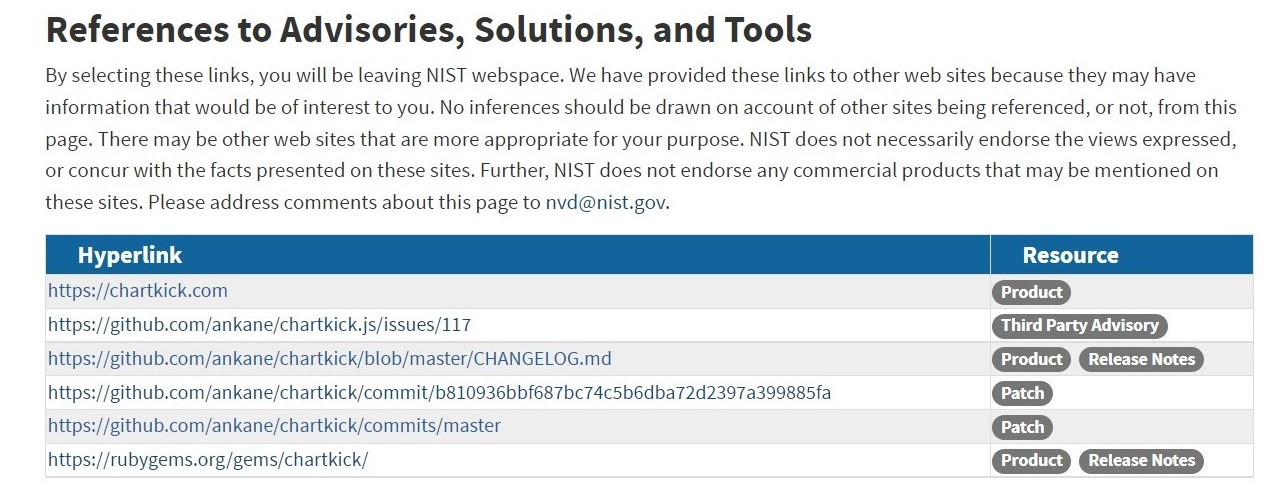
\includegraphics[scale=0.44]{fig/NVD-2019-18841}
    %\vspace{-10pt}
    \caption{NVD平台中漏洞CVE-2019-18841的参考链接}\label{fig:CVE-2019-18841}
\end{figure*}

\textbf{检索GitHub:}检索GitHub中,带有漏洞标识符的代码提交。如图\ref{fig:commitmessage}所示,漏洞CVE-2018-8014的补丁提交信息\footnote{https://github.com/apache/tomcat80/commit/2c9d8433bd3247a2856d4b255}为“Fix https://bz.apache.org/bugzilla/sho\\w\_bug.cgi?id=62343 Make CORS filter defaults more secure. This is the fix for CVE-2018-8014.”,漏洞标识符“CVE-2018-8014”出现在该提交信息中。以“CVE-2018-8014”为输入,通过检索GitHub即可获取该补丁提交。%作为漏洞CVE-2018-8014的补丁。
\begin{figure*}[!t]
    \centering
    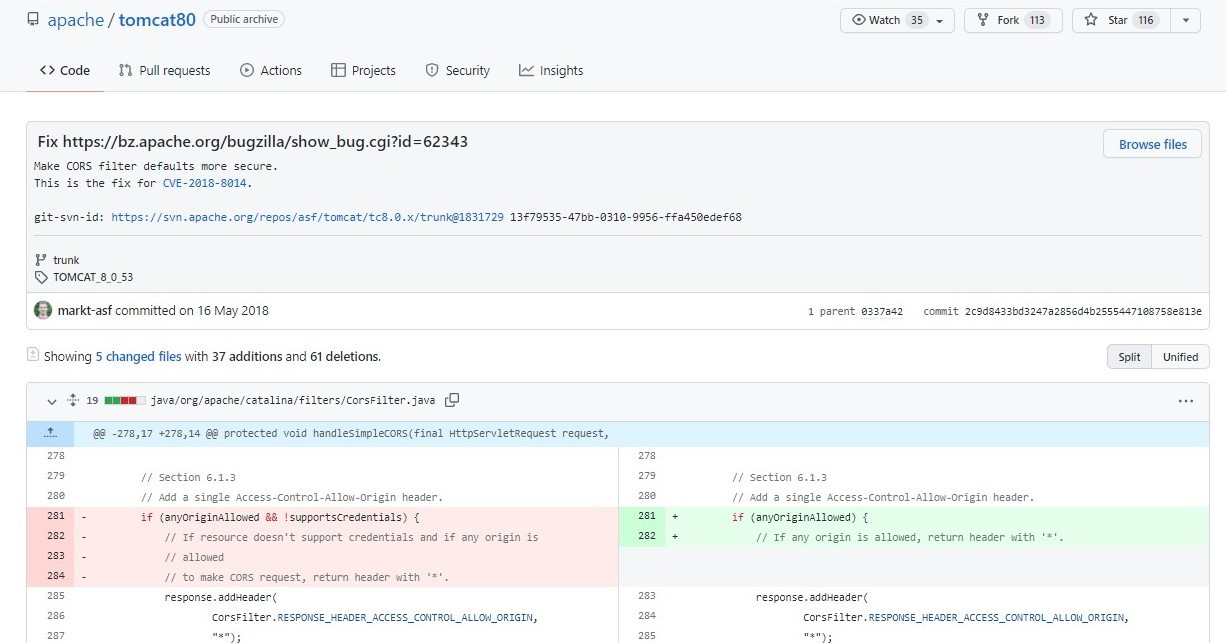
\includegraphics[scale=0.45]{fig/CVE in commit message.jpg}
    %\vspace{-10pt}
    \caption{CVE-2018-8014标识符出现在提交信息中}\label{fig:commitmessage}
\end{figure*}

\textbf{检索NVD以及GitHub:}将前两种方法结合为第三种基于启发式规则的方法,即检索NVD中的参考链接以及GitHub中的代码提交。

\begin{table*}[!t]
    \centering
    % \footnotesize
    \small
    \caption{\tool VS. 基于启发式规则的方法和商业数据库}\label{table:heuristic}
    %\vspace{-10pt}
    \begin{tabular}{|*{1}{C{4.2em}}|*{1}{C{2.0em}}|*{1}{C{4.9em}}*{3}{C{2.0em}}|*{1}{C{4.9em}}*{3}{C{2.0em}}|}
    % \begin{tabular}{|c|c|cccc|cccc|}
    \noalign{\hrule height 1pt}
    \multirow{2}{*}{映射类型} & \multirow{2}{*}{数量} &  \multicolumn{4}{c|}{\tool} & \multicolumn{4}{c|}{ 检索NVD}\\\cline{3-10}
    & & Coverage & Pre. & Rec. & F1 & Coverage & Pre. & Rec. & F1 \\
    \noalign{\hrule height 1pt}
    1:1 (SP) & 567 &	465 (82.0\%) & 0.860 & 0.951 & 0.881    & 282 (49.7\%) & 0.973 & 0.986 & 0.977 \\
    1:$i$ (MEP) &195 &	189 (96.9\%) & 0.886 & 0.918 & 0.888       & 70 (35.9\%) & 0.932 & 0.925 & 0.921 \\
    1:$n$ (MP) & 101 &	81 (80.2\%) & 0.872 & 0.741 & 0.761     & 33 (32.7\%) & 0.980 & 0.552 & 0.683  \\
    1:$n$ (MB) & 372 &	349 (93.8\%) & 0.861 & 0.788 & 0.795      & 148 (39.8\%) & 0.979 & 0.416 & 0.546 \\
    1:$n$ (MR) & 60 &	56 (93.3\%) & 0.831 & 0.620 & 0.659       & 14 (23.3\%) & 1.000 & 0.708 & 0.794  \\\hline
    总计 & 1,295 &	    1,140 (88.0\%) & 0.864 & 0.864 & 0.837    & 527 (40.7\%) & 0.970 & 0.805 & 0.842 \\
    \noalign{\hrule height 1pt}
    \multirow{2}{*}{映射类型} & \multirow{2}{*}{数量} &  \multicolumn{4}{c|}{检索GitHub} & \multicolumn{4}{c|}{检索NVD以及GitHub}\\\cline{3-10}
    & & Coverage & Pre. & Rec. & F1 & Coverage & Pre. & Rec. & F1 \\
    \noalign{\hrule height 1pt}
    1:1 (SP) & 567 &	95 (16.8\%) & 0.416 & 0.642 & 0.471    & 345 (60.8\%) & 0.839 & 0.930 & 0.864 \\
    1:$i$ (MEP) &195 &	33 (16.9\%) & 0.472 & 0.490 & 0.452    & 91 (46.7\%) & 0.821 & 0.867 & 0.820 \\
    1:$n$ (MP) & 101 &	28 (27.8\%) & 0.536 & 0.445 & 0.461     & 49 (48.5\%) & 0.779 & 0.605 & 0.647  \\
    1:$n$ (MB) & 372 &	126 (33.9\%) & 0.445 & 0.236 & 0.284    & 201 (54.0\%) & 0.704 & 0.393 & 0.465 \\
    1:$n$ (MR) & 60 &	23 (38.3\%) & 0.627 & 0.345 & 0.413     & 33 (55.0\%) & 0.801 & 0.539 & 0.604  \\\hline
    总计 & 1,295 &	    305 (23.6\%) & 0.461 & 0.417 & 0.386    & 719 (55.5\%) & 0.793 & 0.732 & 0.720 \\
    \noalign{\hrule height 1pt}
    \multirow{2}{*}{映射类型} & \multirow{2}{*}{数量} &  \multicolumn{4}{c|}{$DB_A$} & \multicolumn{4}{c|}{$DB_B$}\\\cline{3-10}
    & & Coverage & Pre. & Rec. & F1 & Coverage & Pre. & Rec. & F1 \\
    \noalign{\hrule height 1pt}
    1:1 (SP) & 567       & 100.0\% & 0.908 & 0.915 & 0.910  & 100.0\% & 0.900 & 0.921 & 0.906   \\
    1:$i$ (MEP) & 195    & 100.0\% & 0.935 & 0.898 & 0.902  & 100.0\% & 0.924 & 0.909  & 0.906   \\
    1:$n$ (MP) & 101     & 100.0\% & 0.923 & 0.483 & 0.616  & 100.0\% & 0.911 & 0.520 & 0.638    \\
    1:$n$ (MB) & 372     & 100.0\% & 0.941 & 0.510 & 0.620  & 100.0\% & 0.932 & 0.436 & 0.555    \\
    1:$n$ (MR) & 60      & 100.0\% & 0.913 & 0.610 & 0.695  & 100.0\% & 0.964 & 0.526 & 0.636   \\\hline
    总计 & 1,295        & 100.0\% & 0.923 & 0.748 & 0.793  & 100.0\% & 0.917 & 0.730 & 0.771     \\
    \noalign{\hrule height 1pt}
    \end{tabular}
\end{table*}

表\ref{table:heuristic}显示了三种基于启发式规则的方法与\tool 的准确率对比结果。

\textbf{补丁覆盖率方面:}可以发现,在包含1,295个漏洞的的深度数据集上,三种基于启发式规则方法的补丁覆盖率都较低。对于基于检索NVD的启发式方法,\tocheck{768(59.3\%)}的漏洞无法找到补丁,补丁覆盖率为40.7\%。对于基于检索GitHub的启发式方法,\tocheck{990(76.4\%)}的漏洞无法找到补丁,补丁覆盖率为23.6\%。对于基于检索NVD以及GitHub的启发式方法,\tocheck{576(44.5\%)}的漏洞无法找到补丁,补丁覆盖率为55.5\%。然而,仅\tocheck{155(12.0\%)}漏洞的补丁无法被\tool 找到,\tool 的补丁覆盖率为88.0\%。

\textbf{补丁准确性方面:}基于检索NVD的启发式方法具有较高的精确率(\tocheck{0.970}),这是因为NVD平台的信息都经过人工核对,参考链接的置信度比较高。但对于一对多映射关系的漏洞,基于检索NVD的启发式方法召回率就比较低,分别为\tocheck{0.552、0.416和0.708}。这也反映出NVD平台漏洞补丁的不完整情况。
与基于检索NVD的启发式方法对比,\tool 的精确率更低,但拥有更高的召回率和相似的F1值.尤其是对于\textit{MP}和\textit{MB}类型的漏洞,\tool 的召回率也明显更高。考虑到\tool 的补丁覆盖率比基于检索NVD的启发式方法多出\tocheck{116.3\%},\tool 中轻微的准确率降低是可以接受的。

基于检索GitHub的方法具有较低的精确率和召回率,分别为\tocheck{0.461}和\tocheck{0.417},而基于检索NVD以及GitHub的方法中和了前两种方法,精确率和召回率分别为\tocheck{0.793}和\tocheck{0.732}。与基于检索GitHub的启发式方法和基于检索NVD以及GitHub的启发式方法对比,\tool 在精确率、召回率和F1值上全面胜出。\tool 的F1值分别高出了\tocheck{116.8\%}和\tocheck{16.3\%}。

% \begin{tcolorbox}[size=title,opacityfill=0.15]
% Highlight:与现有的基于启发式规则的方法相比,\tool 将补丁覆盖率提高\tocheck{58.6\%}到\tocheck{273.8\%},同时,将F1值提高\tocheck{116.8\%}。
% \end{tcolorbox}
综上,与现有的基于启发式规则的方法相比,\tool 能够显著的提高补丁覆盖率和F1值。\tool 将补丁覆盖率提高\tocheck{58.6\%}到\tocheck{273.8\%},同时,将F1值提高\tocheck{116.8\%}。


\subsection{与商业漏洞数据库对比}
% 考虑到漏洞数据库$DB_A$和$DB_B$并非由工具自动化构建,构建的过程涉及了大量人工工作,并不可知且无法量化,无法进行公平的比较。
% 本节与商业漏洞数据库$DB_A$和$DB_B$进行比较的并非为了证明\tool 或是$DB_A$和$DB_B$的优劣,因为

考虑到漏洞数据库$DB_A$和$DB_B$并非由工具自动化构建,构建的过程涉及了大量人工工作。因此,漏洞数据库$DB_A$和$DB_B$中漏洞知识的质量较高,自动化补丁识别工具难以全面超越。本文将\tool 与数据库$DB_A$和$DB_B$进行对比,可以对比评估\tool 所达到的准确性水平,并探究\tool 用于改进或补充现有的商业漏洞数据库的可能性。%,也能体现\tool 的实用价值。

从表\ref{table:heuristic}可以看出,\tool 能找到补丁的漏洞数比$DB_A$和$DB_B$少了\tocheck{12.0\%},补丁覆盖率仅为88.0\%,且精确率也分别低了\tocheck{6.4\%}和\tocheck{5.8\%}。这是因为漏洞数据库$DB_A$和$DB_B$构建过程中涉及了安全专家的人工工作,许多补丁由人工收集得来,难以被自动化工具找到。此外,收集的补丁还会经过安全专家验证,因此$DB_A$和$DB_B$具有比自动化工具更高的准确率。

此外,\tool 的精确率、召回率和F1值分别为0.864、0.864和0.837,$DB_A$ 的精确率、召回率和F1值分别为0.923、0.748和0.793,$DB_B$ 的精确率、召回率和F1值分别为0.917、0.730和0.771。可以发现\tool 的召回率比$DB_A$和$DB_B$高\tocheck{15.5\%和18.4\%},尤其是对于一对多映射类型的漏洞,\tool 具有更高的召回率。\tool 的F1值也比$DB_A$和$DB_B$高\tocheck{5.5\%和8.6\%}。

这些结果表明,与漏洞数据库$DB_A$和$DB_B$相比,\tool 以略低的补丁精确率和覆盖率为代价,拥有更为显着的召回率。这也说明,\tool 可用于补充现有漏洞数据库缺失的漏洞补丁数据。

% \begin{tcolorbox}[size=title,opacityfill=0.15]
% Highlight:\tool 具有比$DB_A$和$DB_B$高\tocheck{15.5\%和18.4\%}的召回率,以及高\tocheck{5.5\%到8.6\%}的F1值,但同时\tool 牺牲了\tocheck{6.4\%}的精确率和\tocheck{12.0\%}的补丁覆盖率。
% \end{tcolorbox}

\subsection{漏报和误报分析}\label{sec:fpfn}

基于前两节的实验结果,本小节主要分析造成\tool 漏报和误报的原因,即\tool 未找到补丁或找到的补丁不正确的原因。

\textbf{漏报分析:} 漏报是指\tool 未能找到补丁或找全补丁,体现在补丁覆盖率(Coverage)和召回率(Recall)小于1。通过人工分析\tool 未能找到补丁或找全补丁的漏洞数据,本文共总结出造成\tool 漏报的五个主要原因:
\begin{enumerate}
    \item [(1)] 对于一些年代久远的漏洞,NVD、Debian和Red Hat中包含的参考链接比较少,有的参考链接甚至是失效的。这种情况下,\tool 无法构建完整的参考链接网络。例如,对于\tool 未能找到补丁的漏洞CVE-2011-1950,该漏洞有一个关键的参考链接在NVD\footnote{https://nvd.nist.gov/vuln/detail/CVE-2011-1950}中标记为“补丁(Patch)”和“供应商咨询(Vendor Advisory)”。这个链接中很有可能含有补丁,但网址已失效。
    \item [(2)] NVD、Debian和Red Hat平台缺失关键参考链接(如,问题链接),\tool 便难以选出正确的补丁。例如,对于\tool 未能找到补丁的漏洞CVE-2018-14642,该漏洞的问题报告UNDERTOW-1430\footnote{https://issues.redhat.com/browse/UNDERTOW-1430}不包含在任何一个知识源中。人工分析发现,基于这个问题报告可以找到该漏洞的补丁\footnote{https://github.com/undertow-io/undertow/commit/c46b7b49c5a561731c84a76ee52244369af1af8a}。
    \item [(3)] 补丁的提交信息不包含漏洞标识符,但与漏洞描述具有语义相似性。这种情况人工可识别,但自动化工具难以识别。因此,\tool 的参考链接扩增步骤也未能找到这类型的补丁。例如,漏洞CVE-2019-10077\footnote{https://nvd.nist.gov/vuln/detail/CVE-2019-10077},代码提交87c89f@jspwiki\footnote{https://github.com/apache/jspwiki/commit/87c89f0405d6b31fc165358ce5d5bc4536e32a8a}为该漏洞的补丁提交,但提交信息中未提及漏洞标识符,\tool 也未能找到该补丁。
    \item [(4)] GitHub平台提供的用于检索代码提交的REST API仅返回前1,000个结果。如果补丁提交排在1000个以后的话,会使\tool 在\tocheck{参考链接扩增}步骤中错失一些补丁提交。
    \item [(5)] 在补丁选择步骤中,\tool 只选择了具有最高连通度的补丁节点。当其他已包含在参考链接网络中的正确补丁非最高连通度时,会被\tool 遗漏掉,造成漏报。
\end{enumerate}


\textbf{误报分析:}误报是指\tool 识别的结果非该漏洞的补丁,体现在精确率(Precision)小于1。通过人工分析\tool 返回错误补丁的漏洞数据,本文节总结出造成\tool 误报的两个主要原因:

\begin{enumerate}
    \item [(1)] 在讨论和解决漏洞时,相关人员会引用引入漏洞的代码提交(Vulnerability-Inducing Commit)。由于\tool 缺乏对参考链接上下文的语义理解,\tool 会错误地将引入漏洞的代码提交识别为补丁提交。例如,对于漏洞CVE-2020-5249,引入漏洞的代码提交\footnote{https://github.com/ethereum/go-ethereum/commit/fb9f7261ec51e38eedb454594fc19f00de1a6834}和修复漏洞的代码提交\footnote{https://github.com/ethereum/go-ethereum/commit/83e2761c3a13524bd5d6597ac08994488cf872ef}在同一问题报告的评论中被引用,造成了\tool 的误报。
    \item [(2)] 参考链接的页面上列出了多对漏洞及其问题和补丁链接。由于\tool 缺乏语义理解能力,其他漏洞的补丁也可能会被\tool 错误地识别。例如,漏洞CVE-2018-15750的补丁和CVE-2018-15751的补丁都维护在发行说明(Release Note)\footnote{https://docs.saltstack.com/en/latest/topics/releases/2018.3.3.html}中,该发行说明还都被NVD、Debian和Red Hat引用,造成了\tool 的误报。
\end{enumerate}  

% \begin{tcolorbox}[size=title,opacityfill=0.15]
% Highlight:通过人工分析共总结出\tool 漏报的五个主要原因和误报的两个主要原因,针对这些情形,可进一步提高\tool 的准确性。
% \end{tcolorbox}

综上,通过人工分析共总结出\tool 漏报的五个主要原因和误报的两个主要原因。

\section{RQ7:削弱性分析}\label{sec:ablation}

为了探究\tool 中各个步骤及环节设计的实际效果及必要性,本小节通过对比\tool 及其削弱部分环节后生成的变体的准确率,以量化分析各步骤及环节的实际效果。

针对步骤一---参考链接网络构建,本小节分别进行了“去除某一知识源”和“去除网络构建步骤”的削弱处理。针对步骤二---补丁选择,本小节分别进行了“去除基于连通度和置信度的补丁选择方法”、“去除基于连通度或置信度的补丁选择方法”和“变更基于连通度的方法设置”的削弱处理。针对步骤三---补丁扩增,本小节进行了“去除补丁扩增步骤”的削弱处理。表\ref{table:contribution}和\ref{table:contribution-2}为削弱性分析的结果。%,以衡量\tool 中的各步骤和环节对于准确性的贡献度。


\begin{table*}[!t]
    \centering
    \small
    \caption{\tool 削弱性分析结果(1)}\label{table:contribution}
    %\vspace{-10pt}
    \begin{tabular}{|*{1}{C{4.2em}}|*{1}{C{2.0em}}|*{1}{C{4.9em}}*{3}{C{2.0em}}|*{1}{C{4.9em}}*{3}{C{2.0em}}|}
    % \begin{tabular}{|c|c|cccc|cccc|}
    \noalign{\hrule height 1pt}
    \multirow{2}{*}{映射类型} & \multirow{2}{*}{数量} &  \multicolumn{4}{c|}{ \tool } & \multicolumn{4}{c|}{$v_1^1$: \tool w/o NVD} \\\cline{3-10}
    & & Coverage & Pre. & Rec. & F1 & Coverage & Pre. & Rec. & F1  \\
    \noalign{\hrule height 1pt}
    1:1 (SP) & 567 &	465 (82.0\%) & 0.860 & 0.951 & 0.881 &	281 (49.6\%) & 0.820 & 0.936 & 0.846  \\
    1:$i$ (MEP) &195 &	189 (96.9\%) & 0.886 & 0.918 & 0.888 &	    116 (59.5\%) & 0.882 & 0.935 & 0.886 	 \\
    1:$n$ (MP) & 101 &	81 (80.2\%) & 0.872 & 0.741 & 0.761 &	60 (59.4\%) & 0.881 & 0.728 & 0.766 	 \\
    1:$n$ (MB) & 372 &	349 (93.8\%) & 0.861 & 0.788 & 0.795 &	288 (77.4\%) & 0.876 & 0.780 & 0.800 	 \\
    1:$n$ (MR) & 60 &	56 (93.3\%) & 0.831 & 0.620 & 0.659 &	    52 (86.7\%) & 0.848 & 0.551 & 0.624 	 \\\hline
    总计 & 1,295 &	    1,140 (88.0\%) & 0.864 & 0.864 & 0.837 &	797 (61.5\%) & 0.856 & 0.839 & 0.815 	 \\
    \noalign{\hrule height 1pt}

    \multirow{2}{*}{映射类型} & \multirow{2}{*}{数量} &  \multicolumn{4}{c|}{$v_1^2$: \tool w/o Debian} & \multicolumn{4}{c|}{$v_1^3$: \tool w/o Red Hat} \\\cline{3-10}
    & & Coverage & Pre. & Rec. & F1 & Coverage & Pre. & Rec. & F1   \\
    \noalign{\hrule height 1pt}
    1:1 (SP) & 567 &	457 (80.6\%) & 0.847 & 0.943 & 0.869 &	454 (80.1\%) & 0.853 & 0.943 & 0.874 \\
    1:$i$ (MEP) &195 &	187 (95.6\%) & 0.880 & 0.912 & 0.882 &	    188 (96.4\%) & 0.883 & 0.918 & 0.886 \\
    1:$n$ (MP) & 101 &	79 (78.2\%) & 0.851 & 0.716 & 0.739 &	80 (79.2\%) & 0.880 & 0.736 & 0.760 \\
    1:$n$ (MB) & 372 &	344 (92.5\%) & 0.838 & 0.760 & 0.771 &	337 (90.6\%) & 0.844 & 0.761 & 0.767 \\
    1:$n$ (MR) & 60 &	55 (91.7\%) & 0.819 & 0.613 & 0.651 &	    56 (93.3\%) & 0.738 & 0.640 & 0.618 \\\hline
    总计 & 1,295 &	    1,122 (86.6\%) & 0.848 & 0.849 & 0.821 &	1,115 (86.1\%) & 0.851 & 0.853 & 0.823 \\
    \noalign{\hrule height 1pt}
    
    \multirow{2}{*}{映射类型} & \multirow{2}{*}{数量}  & \multicolumn{4}{c|}{$v_1^4$: \tool w/o GitHub} & \multicolumn{4}{c|}{$v_1^5$: \congyingEdit{\tool w/o Network}} \\\cline{3-10}
    & & Coverage & Pre. & Rec. & F1 & Coverage & Pre. & Rec. & F1  \\
    \noalign{\hrule height 1pt}
    1:1 (SP) & 567 &	418 (73.7\%) & 0.898 & 0.943 & 0.908 &	390 (68.8\%) & 0.910 & 0.972 & 0.925 \\
    1:$i$ (MEP) &195 &	176 (90.3\%) & 0.887 & 0.921 & 0.892 &	117 (60.0\%) & 0.956 & 0.959 & 0.941 \\
    1:$n$ (MP) & 101 &	73 (72.3\%) & 0.873 & 0.690 & 0.726 &	61 (60.4\%) & 0.943 & 0.669 & 0.743 \\
    1:$n$ (MB) & 372 &	333 (89.5\%) & 0.874 & 0.752 & 0.773 &	263 (70.7\%) & 0.908 & 0.575 & 0.659 \\
    1:$n$ (MR) & 60 &	53 (88.3\%) & 0.816 & 0.545 & 0.604 &	50 (83.3\%) & 0.920 & 0.641 & 0.712 \\\hline
    总计 & 1,295 &	    1,053 (81.3\%) & 0.883 & 0.841 & 0.835 &	881 (68.0\%) & 0.918 & 0.812 & 0.823 \\
    \noalign{\hrule height 1pt}
    \end{tabular}
\end{table*}

\subsection{去除某一知识源} 
在\tool 的步骤一(参考链接网络构建)中,通过分别删除四个知识源NVD、Debian、Red Hat和GitHub中的一个,生成削弱后的变体$v_1^1$、$v_1^2$、$v_1^3$和$v_1^4$。如表\ref{table:contribution}所示,这四个变体的补丁覆盖率都小于\tool 。在精确率、召回率和F1值相当的情况下,$v_1^1$、$v_1^2$、$v_1^3$和$v_1^4$未找到补丁的漏洞数分别为498(38.5\%)、173(13.4\%)、180(13.9\%)和242(18.7\%),比\tool 分别多了\tocheck{30.1\%、1.6\%、2.2\%和7.6\%}。这表明,集成更多的知识源,构建更完整的参考链接网络,有助于取得更好的补丁识别结果。\tool 中选取的四个知识源都有助于构建更完整的参考链接网络,也更有助于为更多的漏洞找到补丁。同时,可以发现,删除知识源NVD和GitHub后未找到补丁的漏洞数增到了498(38.5\%)和242(18.7\%),补丁覆盖率减少到了61.5\%和81.3\%。这也说明知识源NVD和GitHub的贡献度是最高的,效果也是最好的。

\subsection{去除网络构建步骤}
在\tool 的步骤一(参考链接网络构建)中,通过不以逐层迭代的方式构建参考链接网络,而是仅仅使用包含在四个知识源公告中直接引用的参考链接,生成削弱后的变体$v_1^5$。具体实现为,在\tool 的步骤一中跳过“参考链接分析”环节,实验结果为表\ref{table:contribution}中的$v_1^5$。可以发现,$v_1^5$没有找到补丁的漏洞数量增加到了414(32.0\%),补丁覆盖率下降到了68.0\%。但同时精确率却高出了\tocheck{6.3\%},召回率低了\tocheck{6.0\%},F1值较为相似。这些结果表明,补丁并不总是在NVD、Debian和Red Hat中被直接引用,而是可能隐藏在多层参考链接之中,去除网络中深层参考链接后,会丢失补丁。同时说明,本文构建的参考链接网络有助于用户找到隐藏的补丁,但需要以小幅的精确率降低为代价。

\begin{table*}[!t]
    \centering
    \small
    \caption{\tool 削弱性分析结果(2)}\label{table:contribution-2}
    %\vspace{-10pt}
    \begin{tabular}{|*{1}{C{4.2em}}|*{1}{C{2.0em}}|*{1}{C{4.9em}}*{3}{C{2.0em}}|*{1}{C{4.9em}}*{3}{C{2.0em}}|}
    % \begin{tabular}{|c|c|cccc|cccc|}
    \noalign{\hrule height 1pt}
    
    \multirow{2}{*}{映射类型} & \multirow{2}{*}{数量} &  \multicolumn{4}{c|}{$v_2^1$: \congyingEdit{\tool w/o Selection}} & \multicolumn{4}{c|}{$v_2^2$: \tool w/o Connectivity} \\\cline{3-10}
    & & Coverage & Pre. & Rec. & F1 & Coverage & Pre. & Rec. & F1 \\
    \noalign{\hrule height 1pt}
    1:1 (SP) & 567 &	465 (82.0\%) & 0.632 & 0.961 & 0.680 &	322 (56.8\%) & 0.892 & 0.978 & 0.913  \\
    1:$i$ (MEP) &195 &	189 (96.9\%) & 0.622 & 0.976 & 0.682 &	    84 (43.1\%) & 0.929 & 0.939 & 0.915  \\
    1:$n$ (MP) & 101 &	81 (80.2\%) & 0.615 & 0.933 & 0.656 &	45 (44.6\%) & 0.953 & 0.685 & 0.764  \\
    1:$n$ (MB) & 372 &	349 (93.8\%) & 0.616 & 0.903 & 0.657 &	181 (48.7\%) & 0.927 & 0.787 & 0.821  \\
    1:$n$ (MR) & 60 &	56 (93.3\%) & 0.368 & 0.891 & 0.394 &	    33 (55.0\%) & 0.885 & 0.722 & 0.772  \\\hline
    总计 & 1,295 &	1,140 (88.0\%) & 0.611 & 0.940 & 0.658 &	    665 (51.4\%) & 0.910 & 0.889 & 0.871  \\
    \noalign{\hrule height 1pt}

    \multirow{2}{*}{映射类型} & \multirow{2}{*}{数量} & \multicolumn{4}{c|}{$v_2^3$: \tool w/o Confidence} &  \multicolumn{4}{c|}{$v_2^4$: \tool with Path Length} \\\cline{3-10}
    & & Coverage & Pre. & Rec. & F1 & Coverage & Pre. & Rec. & F1 \\
    \noalign{\hrule height 1pt}
    1:1 (SP) & 567 &	465 (82.0\%) & 0.860 & 0.942 & 0.879  & 465 (82.0\%) & 0.833 & 0.957 & 0.859\\
    1:$i$ (MEP) &195 &	189 (96.9\%) & 0.888 & 0.913 & 0.889 &     189 (96.9\%) & 0.848 & 0.945 & 0.867 \\
    1:$n$ (MP) & 101 &	81 (80.2\%) & 0.880 & 0.722 & 0.751 &   81 (80.2\%) & 0.849 & 0.760 & 0.742\\
    1:$n$ (MB) & 372 &	349 (93.8\%) & 0.871 & 0.765 & 0.784 &    349 (93.8\%) & 0.830 & 0.798 & 0.770\\
    1:$n$ (MR) & 60 &	56 (93.3\%) & 0.849 & 0.462 & 0.550 &     56 (93.3\%) & 0.652 & 0.747 & 0.590 \\\hline
    总计 & 1,295 &	    1,140 (88.0\%) & 0.869 & 0.844 & 0.826 &  1,140 (88.0\%) & 0.827 & 0.882 & 0.812 \\
    \noalign{\hrule height 1pt}

    
    \multirow{2}{*}{映射类型} & \multirow{2}{*}{数量} &   \multicolumn{4}{c|}{$v_2^5$: \tool with Path Number} & \multicolumn{4}{c|}{$v_3$: \tool w/o Expansion} \\\cline{3-10}
    & & Coverage & Pre. & Rec. & F1 & Coverage & Pre. & Rec. & F1 \\
    \noalign{\hrule height 1pt}
    1:1 (SP) & 567 &	465 (82.0\%) & 0.805 & 0.951 & 0.837 &  465 (82.0\%) & 0.871 & 0.948 & 0.889\\
    1:$i$ (MEP) &195 &	189 (96.9\%) & 0.849 & 0.920 & 0.858 &     189 (96.9\%) & 0.910 & 0.914 & 0.902\\
    1:$n$ (MP) & 101 &	81 (80.2\%) & 0.801 & 0.756 & 0.726 &   81 (80.2\%) & 0.873 & 0.696 & 0.732\\
    1:$n$ (MB) & 372 &	349 (93.8\%) & 0.833 & 0.811 & 0.791 &    349 (93.8\%) & 0.860 & 0.506 & 0.590\\
    1:$n$ (MR) & 60 &	56 (93.3\%) & 0.789 & 0.630 & 0.644 &     56 (93.3\%) & 0.847 & 0.567 & 0.629\\\hline
    总计 & 1,295 &	    1,140 (88.0\%) & 0.819 & 0.873 & 0.809 &  1,140 (88.0\%) & 0.873 & 0.771 & 0.776\\
    \noalign{\hrule height 1pt}
    \end{tabular}
\end{table*}

\subsection{去除补丁选择步骤}
\textbf{去除基于连通度和置信度的补丁选择方法:}
在\tool 的步骤二(补丁选择)中,通过选择网络中的所有补丁,而非选择具有高置信度的补丁和具有高连通度的补丁,生成的变体$v_2^1$(见表\ref{table:contribution-2})。可以发现,该变体显着提高了\tool 的召回率,由0.864提高到了0.940多了\tocheck{8.8\%},尤其是对于一对多映射类型的漏洞。但同时精确率大幅下降\tocheck{29.3\%},由0.864降到了0.611;F1值也大幅下降了\tocheck{21.4\%},由0.837降到了0.658。该结果表明,参考链接网络中确实包含了大部分漏洞的正确补丁,且基于连通度和置信度的补丁选择方法有助于实现精确率和召回率之间的平衡。

\textbf{去除基于连通度或置信度的补丁选择方法:}
在\tool 的步骤二(补丁选择)中,并非选择具有高置信度和连通度的补丁,而是采用两个补丁选择方法之一,即选择具有高置信度或连通度的补丁,生成两个变体$v_2^2$和$v_2^3$。

在不使用基于连通度的补丁选择方法时,$v_2^2$找到补丁的漏洞数比\tool 少了\tocheck{41.7\%},覆盖率下降到了51.4\%,但同时精确率提升了\tocheck{5.3\%},召回率提高了\tocheck{2.9\%},F1值提高了\tocheck{4.1\%}。这些结果表明,基于连通度的补丁选择方法有助于为更多漏洞找到补丁,但同时也会引入少部分噪声。

在不使用基于置信度的补丁选择方法时,$v_2^3$的召回率和F1值会略有下降,分别由0.864和0.837降到了0.844和0.826;尤其是对于\textit{MR}类型的漏洞,影响更为明显,召回率由0.620下降到0.462。这些结果表明,基于置信度的补丁选择方法有助于为漏洞找到更多的补丁,且几乎不会引入少噪声。

%这些结果表明,基于置信度的补丁选择方法有助于在所有评估标准(Coverage、Precision、Recall和F1-Score)之间实现平衡的准确性。

\textbf{变更基于连通度的方法设置:}
在\tool 的步骤二(补丁选择)基于连通度的补丁选择方法中,通过仅考虑路径长度(即选择到根节点的路径最短的补丁)或仅考虑路径数量(即选择具有最多路径数的补丁)来削弱基于连通度的补丁选择方法,分别生成了变体$v_2^4$和$v_2^5$。

可以发现,$v_2^4$和$v_2^5$的精确率分别比\tool 低了\tocheck{4.3\%}和\tocheck{5.2\%},召回率分别高了\tocheck{2.1\%}和\tocheck{1.0\%},F1值分别降低了\tocheck{3.0\%}和\tocheck{3.3\%}。这些结果表明,基于连通度的补丁选择方法中所设计的补丁节点到根节点的路径长度和路径数都有助于提高\tool 的准确率,但同时会使召回率略微降低。

\subsection{去除补丁扩增步骤}
去除\tool 的步骤三(补丁扩增)后,生成变体$v_3$。可以发现,$v_3$的召回率为0.771,比\tool 的召回率下降了\tocheck{10.8\%}。$v_3$的F1值为0.776,比\tool 的F1值下降了\tocheck{7.3\%}。尤其是对于一对多映射类型的漏洞,召回率和F1值下降更为显著。这些结果表明,补丁扩增步骤有助于\tool 更完整地为漏洞找到多个补丁。

% \begin{tcolorbox}[size=title,opacityfill=0.15]
% Highlight:\tool 中的知识源、网络构建、补丁选择和补丁扩增步骤及其中的设计都具有一定的效果和必要性,都对\tool  补丁识别的准确性做出了贡献。
% \end{tcolorbox}
综上,\tool 中的知识源、网络构建、补丁选择和补丁扩增步骤的设计对最终结果都有一定的贡献度和必要性。


\section{RQ8:敏感度分析}\label{sec:sensitivity}
% \begin{figure*}[h]
%     \centering
%     \begin{subfigure}[b]{0.45\textwidth}
%     \centering
%     \includegraphics[scale=0.55]{fig/rq8-sensitivity-depth.pdf}
%     %\vspace{-5pt}
%     \caption{网络深度限制}\label{fig:depth}
%     \end{subfigure}
%     \begin{subfigure}[b]{0.45\textwidth}
%     \centering
%     \includegraphics[scale=0.55]{fig/rq8-sensitivity-span.pdf}
%     %\vspace{-5pt}
%     \caption{提交时间跨度}\label{fig:span}
%     \end{subfigure}
%     %\vspace{-20pt}
%     \caption{网络深度限制和提交时间跨度的敏感性分析结果}\label{fig:sensitivity}
% \end{figure*}

本小节将评估\tool 的准确性对参数的敏感性,及\tool 中参数设置合理性。\tool 中有两个可配置的参数,分别是:\tool 步骤一网络构建时网络深度限制的设置,以及步骤三补丁扩增时的相关代码提交时间跨度的设定。

在评估\textbf{RQ6 准确性评估}、\textbf{RQ7 削弱性分析}、\textbf{RQ9 通用性分析}和\textbf{RQ10 实用性能分析}时,网络深度限制默认设置为\textbf{5}层,代码提交时间跨度默认设置为\textbf{30}天。为了评估\tool 对这两个参数的敏感性,该小节将固定其中一个参数为默认设置,改变另一个参数的设置,并在深度数据集上重新运行\tool 。网络深度限制具体设置为3、4、5和6层,提交时间跨度具体设置为0、10、20、30、40、50和60天。
\begin{figure*}[!t]
    \centering
    \includegraphics[scale=0.9]{fig/rq8-sensitivity-depth.pdf}
    %\vspace{-5pt}
    \caption{网络深度限制(层数)敏感性分析结果}\label{fig:depth}
\end{figure*}

\begin{figure*}[!t]
    \centering
    \includegraphics[scale=0.9]{fig/rq8-sensitivity-span.pdf}
    %\vspace{-20pt}
    \caption{提交时间跨度的敏感性分析结果}\label{fig:span}
\end{figure*}


图\ref{fig:depth}和\ref{fig:span}分别显示了两个参数对\tool 准确性的影响,其中横坐标表示参数的取值,纵坐标表示\tool 的精确率。总体来看,随着网络层数的增加,网络中将包含更多补丁。此时,\tool 覆盖率在上升,精确率在降低,而召回率和F1值先增加后降低。
基于图\ref{fig:depth}中数据,可以认为网络深度限制设置为5层时,\tool 效果最优。

随着代码提交时间跨度的增加,\tool 会搜索到更广的代码提交。\tool 的精确率也会降低,召回率会提高,F1值先上升后下降。其中,\tool 未找到补丁的漏洞数量并不改变,即补丁覆盖率并未改变,所以没有在图\ref{fig:span}中显示。基于图\ref{fig:span}中数据,可以认为提交时间跨度设置为30天时,\tool 效果最优。

% \begin{tcolorbox}[size=title,opacityfill=0.15]
% Highlight:总的来说,\tool 的精确率对两个可配置参数的变化不是很敏感。
% \end{tcolorbox}
综上,\tool 的准确率对两个可配置参数的变化不是非常敏感,且网络深度参数设置为5层、提交时间跨度设置为30天时效果相对最优。

\section{RQ9:通用性分析}\label{sec:generality}

% \begin{table*}[h]
%     \centering
%     \footnotesize
%     \caption{Generality of \tool over Two Additional Datasets}\label{table:generality}
%     %\vspace{-10pt}
%     % \begin{tabular}{|c|*{1}{C{5.1em}}|*{3}{C{2.6em}}|*{1}{C{5.1em}}*{3}{C{2.5em}}|*{1}{C{5.1em}}*{3}{C{2.5em}}|}
%     \begin{tabular}{|c|c|ccc|cccc|cccc|}   
%     \noalign{\hrule height 1pt}
%     \multirow{2}{*}{Dataset} & \multirow{2}{*}{Number} &  \multicolumn{3}{c|}{\tool} & \multicolumn{4}{c|}{$DB_A$} & \multicolumn{4}{c|}{$DB_B$} \\\cline{3-13}
%     & & Pre. & Rec. & F1 & Coverage & Pre. & Rec. & F1  & Coverage &  Pre. & Rec. & F1 \\
%     \noalign{\hrule height 1pt}
%     First Dataset & 91 & 0.823 & 0.845 & 0.784  & 29 (31.8\%) &  0.935 & 0.827 & 0.858  & 62 (68.1\%) & 0.885 & 0.664 & 0.725\\\hline
%     Second Dataset & 89 & 0.888 & 0.899 & 0.867 & --& -- & -- & -- & -- & -- & -- & -- \\\hline
%     \noalign{\hrule height 1pt}
%     \end{tabular}
% \end{table*}

为了评估\tool 在更大范围开源软件漏洞上的表现(即\tool 的通用性),本节还另外构建了两个漏洞数据集。第一个数据集为,漏洞数据库$DB_A$和$DB_B$中只有一个数据库提供补丁的漏洞(图\ref{fig:rq1-cves-with-patches}中的橙色和蓝色部分),共有\tocheck{3,185}个漏洞。第二个数据集为:两个漏洞数据库$DB_A$和$DB_B$中都没有提供补丁的漏洞(图\ref{fig:rq1-cves-with-patches}在\ref{fig:rq1-cves}中的补集),共有\tocheck{5,468}个漏洞。

在第一个包含\tocheck{3,185}个漏洞的数据集上,\tool 找到了\tocheck{2,155(67.7\%)}漏洞的补丁(补丁覆盖率为67.7\%);而两个漏洞数据库$DB_A$和$DB_B$仅提供了\tocheck{2,190(68.8\%)}和\tocheck{995(31.2\%)}漏洞的补丁。在\tool 找到补丁的\tocheck{2,155}个漏洞中,$DB_A$和$DB_B$仅提供了其中的\tocheck{1,455}和\tocheck{700}个漏洞的补丁。对于第二个数据集中的\tocheck{5,468}个漏洞,\tool 找到了\tocheck{2,816(51.5\%)}漏洞的补丁(补丁覆盖率为51.5\%);而两个漏洞数据库$DB_A$和$DB_B$没有提供补丁,补丁覆盖率为0.0\%。

\begin{table*}[!t]
    \centering
    \small
    \caption{\tool 通用性分析结果}\label{table:generality}
    %\vspace{-10pt}
    % \begin{tabular}{|c|*{1}{C{5.3em}}|*{3}{C{2.4em}}|*{1}{C{5.3em}}|*{3}{C{2.4em}}|}
    \begin{tabular}{|c|c|ccc|c|ccc|}
    \noalign{\hrule height 1pt}
    \multirow{2}{*}{评估对象} &  \multicolumn{4}{c|}{{数据集一 (91个漏洞)}} & \multicolumn{4}{c|}{数据集二(89个漏洞)} \\\cline{2-9}
    & Coverage & Pre. & Rec. & F1 & Coverage & Pre. & Rec. & F1 \\
    \noalign{\hrule height 1pt}
    \tool  & 100.0\% & 0.823 & 0.845 & 0.784      & 100.0\% & 0.888 & 0.899 & 0.867       \\\hline
    $DB_A$  & 62 (68.1\%) &  0.935 & 0.827 & 0.858      & 0.0\% & -- & -- & --        \\\hline
    $DB_B$  & 29 (31.8\%) & 0.885 & 0.664 & 0.725      & 0.0\% & -- & -- & --        \\\hline
    \noalign{\hrule height 1pt}
    \end{tabular}
\end{table*}

此外,本节还从\tool 在第一个和第二个数据集上能找到补丁的漏洞中分别采样了\tocheck{100}个。采用“数据准备”(见章节\ref{sec:preparation})中同样的方式人工找到它们的补丁以评估\tool 的准确性。由于公开的信息有限,人工分析的两份数据集中分别有\tocheck{9}和\tocheck{11}个漏洞不能确定其补丁。

表\ref{table:generality}为评估结果,在第一个数据集取样的\tocheck{91}个漏洞中,\tool 的F1值为\tocheck{0.784},$DB_A$的F1值较高为0.858,$DB_B$的F1值较低为0.725。与小节\ref{sec:accuracy-evaluation}中的结果类似,漏洞数据库$DB_A$和$DB_B$都拥有更高的精确率(0.935和0.885),但召回率也更低(0.827和0.664)。在从第二个数据集取样的\tocheck{89}个漏洞中,$DB_A$和$DB_B$中没有任何漏洞的补丁,而\tool 可取得达到\tocheck{0.867}的F1值,0.888的精确率和0.899的召回率。

这些结果表明,即使对于更大范围的开源软件漏洞,\tool 的准确率也基本稳定。在开源软件漏洞的补丁定位方面,\tool 具有较好的通用性。尤其在第二个数据集上的结果,在漏洞数据库$DB_A$和$DB_B$都没有补丁时,\tool 仍可以找到大量漏洞的补丁。这表明,\tool 可以极大地补充或增强现有的商业漏洞数据库。


% \begin{tcolorbox}[size=title,opacityfill=0.15]
% Highlight:\tool 在两个更大的开源漏洞数据集上可识别到\tocheck{67.7\%}和\tocheck{51.5\%}漏洞的补丁,通过采样评估,精确率分别为\tocheck{0.823}和\tocheck{0.888},召回率分别为\tocheck{0.845}和\tocheck{0.899},体现出\tool 在识别开源漏洞补丁方面具有较好的通用性。
% %\congyingEdit{此外,它还表明\tool可以帮助补充现有的漏洞数据库。}
% \end{tcolorbox}

\section{RQ10: 实用性分析}\label{sec:usefulness}
本小节旨在评估\tool 在实际工作场景下的实用性。在实际工作中,安全专家在使用较准确的自动工具识别到补丁后,他们仍然需要对补丁进行多次确认,以确保补丁的准确性。为了评估\tool 在这种使用场景中的实用性,本文开展了一项用户研究,对比分析用户在有和没有\tool 的辅助下找到10个漏洞补丁的用时和准确性。

本文作者从国内外多所大学和科技公司的安全实验室中共招募了10名实验人员,他们中有软件安全方向的博士后、博士生、硕士研究人员以及工程师。本文还从深度数据集中随机选择了10个漏洞作为实验任务。其中,2个漏洞属于\textit{SP}类型,3个漏洞属于\textit{MEP}类型,1个漏洞属于\textit{MP}类型,4个漏洞属于\textit{MB}类型。为了公平比较,实验人员被平均分为A、B两组。A组人员需要在不使用\tool 的情况下完成前五项任务,并使用\tool 完成剩余的任务。反之,B组人员需要在使用\tool 的情况下完成前5个任务,并不使用\tool 完成剩余的任务。这样可以实现公平比较,在有和没有\tool 时用户完成10项漏洞补丁查找任务的用时和准确性。

% \begin{table*}[h]
%     \centering
%     \footnotesize
%     \caption{用户研究中10个任务的用时和准确率对比结果}\label{table:usefulness}
%     %\vspace{-10pt}
%     \begin{tabular}{|c|*{1}{C{5.3em}}|*{3}{C{2.4em}}|*{1}{C{5.3em}}|*{3}{C{2.4em}}|*{1}{C{5.3em}}|*{3}{C{2.4em}}|}
%     \noalign{\hrule height 1pt}
%     \multirow{2}{*}{Approach} &  \multicolumn{4}{c|}{{All 10 Tasks}} & \multicolumn{4}{c|}{5 Single-Patch Tasks} & \multicolumn{4}{c|}{5 Multiple-Patches Tasks} \\\cline{2-13}
%     & Time (mins) & Pre. & Rec. & F1 & Time (mins) & Pre. & Rec. & F1 & Time (mins) &  Pre. & Rec. & F1 \\
%     \noalign{\hrule height 1pt}
%     w/o \tool & 5.66 & 0.880 & 0.677 & 0.765      & 5.60 & 0.960 & 0.960 & 0.960        & 5.72 & 0.800 & 0.393 & 0.527 \\\hline
%     with \tool  & 4.66 & 0.983 & 0.920 & 0.951      & 3.84 & 1.000 & 1.000 & 1.000        & 5.48 & 0.967 & 0.840 & 0.899 \\\hline
%     \noalign{\hrule height 1pt}
%     \end{tabular}
% \end{table*}

\begin{table*}[!t]
    \centering
    \small
    \caption{用户研究中任务的用时和准确率}\label{table:usefulness}
    %\vspace{-10pt}
    % \begin{tabular}{|c|*{1}{C{5.3em}}|*{3}{C{2.4em}}|*{1}{C{5.3em}}|*{3}{C{2.4em}}|}
    \begin{tabular}{|c|c|ccc|c|ccc|}
    \noalign{\hrule height 1pt}
    \multirow{2}{*}{任务} &  \multicolumn{4}{c|}{{w/o \tool}} & \multicolumn{4}{c|}{with \tool} \\\cline{2-9}
    & 用时 & Pre. & Rec. & F1 & 用时 & Pre. & Rec. & F1 \\
    \noalign{\hrule height 1pt}
    全部10个任务  & 5.66 mins & 0.880 & 0.677 & 0.765      & 4.66 mins& 0.983 & 0.920 & 0.951        \\\hline
    5单补丁任务  & 5.60 mins & 0.960 & 0.960 & 0.960      & 3.84 mins& 1.000 & 1.000 & 1.000        \\\hline
    5多补丁任务  & 5.72 mins & 0.800 & 0.393 & 0.527      & 5.48 mins& 0.967 & 0.840 & 0.899        \\\hline
    \noalign{\hrule height 1pt}
    \end{tabular}
\end{table*}


表\ref{table:usefulness}显示了10个任务的平均时间消耗和补丁的准确性。本节将属于\textit{SP}和\textit{MEP}类型的5个漏洞归类为\textit{单补丁}任务,将属于\textit{MP}和\textit{MB}类型的5个漏洞归类为\textit{多补丁}任务。总体而言,对于全部10个任务,在\tool 的帮助下,实验人员完成每个任务的用时较少(平均4.66分钟),比在没有\tool 时少用了\tocheck{17.7\%}时间。在\tool 的帮助下,补丁的精确率为0.983,召回率为0.920,F1值为0.951。对比没有\tool 时,分别提高了\tocheck{11.7\%},\tocheck{35.9\%}和\tocheck{24.3\%}。

\textbf{用时方面:}对于5个\textit{单补丁}任务,在\tool 的帮助下,实验人员用时显然更短;但对于5个\textit{多补丁}任务,实验人员用时基本持平。这是因为\tool 为\textit{多补丁}任务返回的参考链接网络比\textit{单补丁}任务的更复杂,实验人员需要花费更多的时间理解参考链接网络,并验证其中的补丁。

\textbf{准确性方面:}在\tool 的帮助下,5个\textit{多补丁}任务的准确度提高也较为显着,但对于5个\textit{单补丁}任务则并不显着。这是因为,\textit{单补丁}任务相比\textit{多补丁}任务较为简单,实验人员无需\tool 的帮助即可完成补丁识别。这也表明,\tool 对于具有多个补丁的开源漏洞作用更为明显。

本文作者还采访了每位实验人员,以获取实验人员对\tool 使用感受的评价。总体来说,实验人员都认为漏洞的参考链接网络具有较高的价值,因为它囊括了来自多个知识源的信息,其中不同类型的节点和关系有助于人工定位和验证补丁。一家来自国际知名科技公司的安全工程师评论:\textit{``参考链接网络作为一个证据链,有助于定位和验证补丁"}。此外,实验人员还建议:\tool 可以添加更多的知识源,并提供更多关于补丁节点的信息,如提交消息、代码变更内容等,这些信息有助于人工审查和确认补丁。

% \begin{tcolorbox}[size=title,opacityfill=0.15]
% Highlight:在实际使用中,\tool 有助于用户更准确、更快速地识别到补丁。
% \end{tcolorbox}
综上,在实际使用中,\tool 有助于用户更准确、更快速地识别到补丁。

\section{实验结论}
本文从准确性、削弱性、敏感度、通用性及实用性五个方面评估\tool 进行了评估。结果表明:
\begin{enumerate}
    \item [(1)] \textbf{准确性:}\tool 可以达到88.0\%的补丁覆盖率、86.4\%的精确率和86.4\%的召回率。与现有的基于启发式规则的方法相比,\tool 能够显著地提高补丁覆盖率和F1值,将补丁覆盖率提高\tocheck{58.6\%}到\tocheck{273.8\%},将F1值提高\tocheck{116.8\%}。与商业漏洞数据库$DB_A$和$DB_B$相比,\tool 以略低的补丁精确率和覆盖率为代价,拥有更为显着的召回率。这表明,\tool 可用于补充现有漏洞数据库缺失的漏洞补丁数据。
    \item [(2)] \textbf{削弱性:}\tool 中的知识源、网络构建、补丁选择和补丁扩增步骤的设计对最终结果都有一定的贡献度和必要性。
    \item [(3)] \textbf{敏感度:}\tool 的准确率对两个可配置参数的变化不是非常敏感,且网络深度参数设置为5层、提交时间跨度设置为30天时效果相对最优。
    \item [(4)] \textbf{通用性:}在更大范围的开源软件漏洞上,\tool 具有较好的通用性,覆盖率和准确率比较稳定。在商业漏洞数据库$DB_A$和$DB_B$都没有补丁时,\tool 仍可以找到大量漏洞的补丁。这表明,\tool 可以极大地补充或增强现有的商业漏洞数据库。
    \item [(5)] \textbf{实用性:}在实际工作场景下,\tool 有助于用户更准确、更快速地识别到补丁。
\end{enumerate}

\section{讨论}
基于上文实验评估的结果,以及\tool 的设计,本节将主要讨论\tool 存在的短板和潜在的价值。
\subsection{\tool 的局限性}
\tool 以CVE ID作为输入,因此该方法不适用于没有CVE ID的开源漏洞(即不在CVE平台中的开源漏洞),比如一些秘密修补的漏洞并没有收录在CVE平台中,也没有CVE ID。针对这种情况,一种可能的解决方案是将Advisory ID作为\tool 的输入。

\tool 仅仅包含Debian、Red Hat和GitHub三个次级知识源,也因此会遗漏在其他知识源中出现的补丁。但\tool 具有较好的可扩展性,它可以灵活地扩增其他知识源(如,SecurityFocus\footnote{https://www.securityfocus.com})。

此外,章节\ref{sec:fpfn}中阐述了造成\tool 漏报和误报的多个原因,针对这些原因,可进一步提高\tool 的准确性。。

\subsection{\tool 的价值}
\tool 有益于软件安全领域相关的社区、学术界和工业界。对于安全社区而言,\tool 可以发现缺少补丁的漏洞,并向CVE管理员报告该情况,以提高CVE的信息质量并加速CVE条目的更新,使得CVE、NVD平台的广大用户受益。对于学术界而言,\tool 可以为大规模数据驱动的安全分析工作(例如,基于学习的漏洞检测\cite{li2018vuldeepecker,zhou2019devign})和经验研究工作提供的补丁数据作为研究基础。%它还可以帮助通过分析漏洞补丁以确定受影响组件的工作\cite{dong2019towards}。
对于工业界来说,\tool 可以帮助安全工程师提高商业漏洞数据库的补丁覆盖率和准确性,从而提高软件安全服务的表现。值得一提的是,\tool 已经部署到一家国际知名科技公司。%但是,由于保密协议,本文不便分享相关数据。